\section{Практычны занятак №3}

\subsection{Структура праекта}

На малюнку \ref{img: pz3} прадстаўлена файлавая структура праекта.

\begin{figure}[h!]
\centering
\begin{subfigure}{0.5\textwidth}
    \centering
    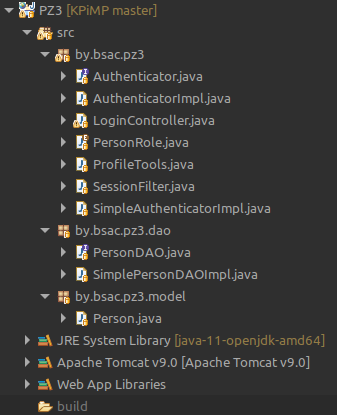
\includegraphics[width=\textwidth]{pz3_structure_1}
\end{subfigure}%
\begin{subfigure}{0.5\textwidth}
    \centering
    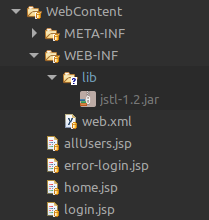
\includegraphics[width=0.7\textwidth]{pz3_structure_2}
\end{subfigure}
\caption{Файлавая структура практычнага занятку}
\label{img: pz3} 
\end{figure}

Заўважце, што ў \textit{WEB-INF/lib} з'явіўся новы файл
\textit{jstl-1.2.jar}. Гэты файл неабходны для магчымасці
карыстацца JSTL тэгамі.

Перад выкананнем задання загрузіць дадзеную бібліятэку
(\textit{jstl-1.2.jar}) і пакладзіце ў дырэкторыю згодна
з малюнкам \ref{img: pz3}.

\subsection{Заданне з тэорыі}

Дадзенае заданне выконваецца на базе практычнага занятку №1
(заданне з тэорыі).

\subsubsection{Апіcанне задання.}

Дабаўце ў вэб-праграму, распрацаваную на першым практычным занятку,
клас, які захоўвае інфармацыю пра карыстальнікаў. Змяніце код
вэб-праграмы для аўтарызацыі пры дапамозе новага класа.
Дабаўце новую старонку, на якой будуць выводзіцца інфармацыя пра ўсіх
магчымых карыстальнікаў.

\subsection{Зыходны код. JSP-старонкі}

\subsubsection{Абноўленая старонка home.jsp.}

Дабавім ўмову \textit{if} для стварэння спасылкі на старонку
\textit{allUsers.jsp}, калі бягучы карыстальнік --- Адміністратар.

У лістынку \ref{lst: pz3_home} прадстаўлена абноўленая старонка
\textit{home.jsp}.

\lstinputlisting[caption={Зыходны код для home.jsp},%
                 label={lst: pz3_home},%
                 language=HTML5,%
                 style=htmlcssjs]{PZ3/JSP/home.jsp}

\subsection{Старонка allUsers.jsp.}

Дадзеная старонка выводзіць у выглядзе табліцы
інфармацыю пра ўсіх магчымых карыстальнікаў (глядзі клас
\textit{SimplePersonDAOImpl}.

У лістынку \ref{lst: pz3_allUsers} прадстаўлена старонка
\textit{allUsers.jsp}.

\lstinputlisting[caption={Зыходны код для allUsers.jsp},%
                 label={lst: pz3_allUsers},%
                 language=HTML5,%
                 style=htmlcssjs]{PZ3/JSP/allUsers.jsp}

\subsection{Зыходны код. Java}

\subsubsection{Пералік PersonRole.}

Для вызначэння ролі карыстальніка выкарыстоўваецца пералік PersonRole.
У ім вызначаюцца дазволеныя назвы для ролі.

У лістынгу \ref{lst: pz3_personRole} прадстаўлены зыходны код пераліку \textit{PersonRole}.

\lstinputlisting[caption={Зыходны код пераліку PersonRole},%
                 label={lst: pz3_personRole},%
                 language=java]{PZ3/Java/PersonRole.java}

\vspace{-\baselineskip}
\subsubsection{Клас Person}

Клас \textit{Person} захоўвае інфармацыю пра карыстальніка.

У лістынгу \ref{lst: pz3_person} прадстаўлены зыходны код класа \textit{Person}.

\lstinputlisting[caption={Зыходны код класа Person},%
                 label={lst: pz3_person},%
                 language=java]{PZ3/Java/Person.java}

\vspace{-\baselineskip}
\subsubsection{Інтэрфейс PersonDAO.}

Інтэрфейс \textit{PersonDAO} вызначае метады, якія неабходна
будзе рэалізаваць у класе \textit{Simp\-le\-Per\-son\-DAO\-Impl}.

У лістынгу \ref{lst: pz3_personDAO} прадстаўлены зыходны код інтэрфейса \textit{PersonDAO}.

\lstinputlisting[caption={Зыходны код інтэрфейса PersonDAO},%
                 label={lst: pz3_personDAO},%
                 language=java]{PZ3/Java/PersonDAO.java}

\vspace{-\baselineskip}
\subsubsection{Клас SimplePersonDAOImpl.}

Дадзены клас захоўвае інфармацыю пра карыстальнікаў,
якія могуць аўтэнтыфікавацца ў вэб-праграме, і магчымасці
пошуку карыстальнікаў па іх даным.

У лістынгу \ref{lst: pz3_simplePersonDAOImpl} прадстаўлены зыходны код класа \textit{SimplePersonDAOImpl}.

\lstinputlisting[caption={Зыходны код класа SimplePersonDAOImpl},%
                 label={lst: pz3_simplePersonDAOImpl},%
                 language=java]{PZ3/Java/SimplePersonDAOImpl.java}

\subsubsection{Абноўлены інтэрфейс Authenticator.}

Абнавім інтэрфейс \textit{Authenticator} для таго,
каб ён мог працаваць з класам Person.

У лістынгу \ref{lst: pz3_authenticator} прадстаўлены зыходны код абноўленага інтэрфейса \textit{Authenticator}.

\lstinputlisting[caption={Зыходны код інтэрфейса Authenticator},%
                 label={lst: pz3_authenticator},%
                 language=java]{PZ3/Java/Authenticator.java}

\subsubsection{Абноўлены клас AuthenticatorImpl.}

Абнавім клас \textit{AuthenticatorImpl}, каб ён ствараў аб'ект
класа Person з інфармацыяй пра карыстальніка па ўмаўчанню.
Зменім логіку метадаў аўтэнтыфікацыі, каб яны вярталі аб'ект
класа Person.

У лістынгу \ref{lst: pz3_authenticatorImpl} прадстаўлены зыходны код абноўленага класа \textit{AuthenticatorImpl}.

\lstinputlisting[caption={Зыходны код класа AuthenticatorImpl},%
                 label={lst: pz3_authenticatorImpl},%
                 language=java]{PZ3/Java/AuthenticatorImpl.java}

\subsubsection{Клас SimpleAuthenticatorImpl.}

Дадзены клас прадастаўляе метады аўтэнтыфікацыі для новага спосабу
захоўвання карыстальнікаў (класы Person і SimplePersonDAOImpl).


У лістынгу \ref{lst: pz3_simpleAuthenticatorImpl} прадстаўлены зыходны код класа \textit{SimpleAuthenticatorImpl}.

\lstinputlisting[caption={Зыходны код класа SimpleAuthenticatorImpl},%
                 label={lst: pz3_simpleAuthenticatorImpl},%
                 language=java]{PZ3/Java/SimpleAuthenticatorImpl.java}

\subsubsection{Абноўлены клас LoginController.}

Абнавім клас \textit{LoginController}, каб ён працаваў з класам
\textit{Person} і ў залежнасці ад ролі карыстальніка дабаўляў
неабходную інфармацыю ў параметры сесіі з уласцівасцяў аб'екта.

У лістынгу \ref{lst: pz3_loginController} прадстаўлены зыходны код абноўленага класа \textit{LoginController}.

\lstinputlisting[caption={Зыходны код класа LoginController},%
                 label={lst: pz3_loginController},%
                 language=java]{PZ3/Java/LoginController.java}

\subsection{Індывідуальнае заданне}

\subsubsection{Апісанне задання.}

У табліцы (глядзі \textit{allUsers.jsp} вывесці паведамленне, што
карыстальнік не ўваходзіў у вэб-праграму, калі дата ўваходу не вызначана,
інакш вывесці дату (для фармавання даты скарыстацца тэгам \textit{fmt}).

Рашэнне дадзенага задання глядзі ў лістынгу \ref{lst: pz3_allUsers}.
